\documentclass[reprint, amsmath, amssymb, aps, pra, nofootinbib]{revtex4-2}

% --- Основные пакеты ---
\usepackage[T2A]{fontenc}
\usepackage[utf8]{inputenc}
\usepackage[russian,english]{babel}

\usepackage{graphicx}
\graphicspath{{figures/}}
\usepackage{bm}

% hyperref в REVTeX лучше подключать с параметрами или использовать встроенный механизм
\usepackage[unicode, colorlinks=true, linkcolor=blue, citecolor=blue, urlcolor=blue]{hyperref}

\begin{document}

\title{3.2.5 (4) Свободные и вынужденные колебания в электрическом контуре}

\author{Ефим Сычев}
\email{sychev.ea@phystech.edu}
\affiliation{Московский физико-технический университет, группа Б02- 506}

\author{Иван Рудко}
\email{rudko.ia@phystech.edu} 
\affiliation{Московский физико-технический университет, группа Б02-506}

\date{\today}
\begin{abstract}
Исследованы свободные и вынужденные колебания в последовательном $RLC$-контуре. Измерена зависимость периода свободных колебаний от ёмкости и логарифмический декремент затухания при разных сопротивлениях, по нему найдено критическое сопротивление. В режиме качания частоты записаны АЧХ и ФЧХ для двух сопротивлений. Добротность контура определена несколькими способами: по ширине резонансной кривой, по ФЧХ, по нарастанию и затуханию колебаний в цуге и по фазовой спирали.
\end{abstract}

\maketitle

% --- Основной текст ---
\section{Введение}
Добротность — главная характеристика колебательного контура: от неё зависит и то, как быстро затухают свободные колебания, и то, насколько острый получается резонанс. В идеальном контуре потерь нет, в реальном они определяются активным сопротивлением, причём не только внешним, но и сопротивлением самой катушки. В работе измерялись параметры последовательного $RLC$-контура (период, декремент затухания, критическое сопротивление) и сравнивались значения добротности, полученные разными независимыми способами.

\section{Физические основы явления}
Свободные колебания в $RLC$-контуре описываются уравнением затухающего осциллятора, и при малом затухании напряжение на конденсаторе — это синусоида с экспоненциально спадающей амплитудой. Период при этом близок к томсоновскому: $T = 2\pi\sqrt{LC}$.
Затухание удобно характеризовать логарифмическим декрементом $\Theta$, который находится по двум амплитудам, разделённым $n$ периодами:
\begin{equation}
\Theta = \frac{1}{n} \ln \frac{U_m}{U_{m+n}}
\label{eq:decrement}
\end{equation}
Если увеличивать сопротивление, то при $R_{cr} = 2\sqrt{L/C}$ колебания пропадают и процесс становится апериодическим. 
Если на контур подать гармоническую ЭДС, в нём устанавливаются вынужденные колебания, и амплитуда $U_C$ максимальна на резонансной частоте $\nu_0$. Добротность можно найти по АЧХ как отношение резонансной частоты к ширине полосы:
\begin{equation}
Q = \frac{\omega_0}{2\Delta\Omega}
\label{eq:q_achx}
\end{equation}
где $2\Delta\Omega$ — ширина кривой на уровне $1/\sqrt{2}$ от максимума.
По ФЧХ ширину $\Delta\omega$ берут на уровне $-\pi/4$ (после отражения нижней ветви относительно $-\pi/2$):
\begin{equation}
Q = \frac{\omega_0}{\Delta\omega}
\label{eq:q_fchx}
\end{equation}
С декрементом добротность связана просто: $Q = \pi / \Theta$. Если же контур возбуждать цугами, то декремент можно найти и по тому, как быстро нарастает амплитуда:
\begin{equation}
\Theta = \frac{1}{n} \ln \frac{U_0 - U_k}{U_0 - U_{k+n}}
\label{eq:decrement_rise}
\end{equation}
здесь $U_0$ — амплитуда установившихся колебаний, $U_k$ и $U_{k+n}$ — амплитуды на участке нарастания.

\section{Экспериментальная установка}

\begin{figure*}[t!]
    \centering
    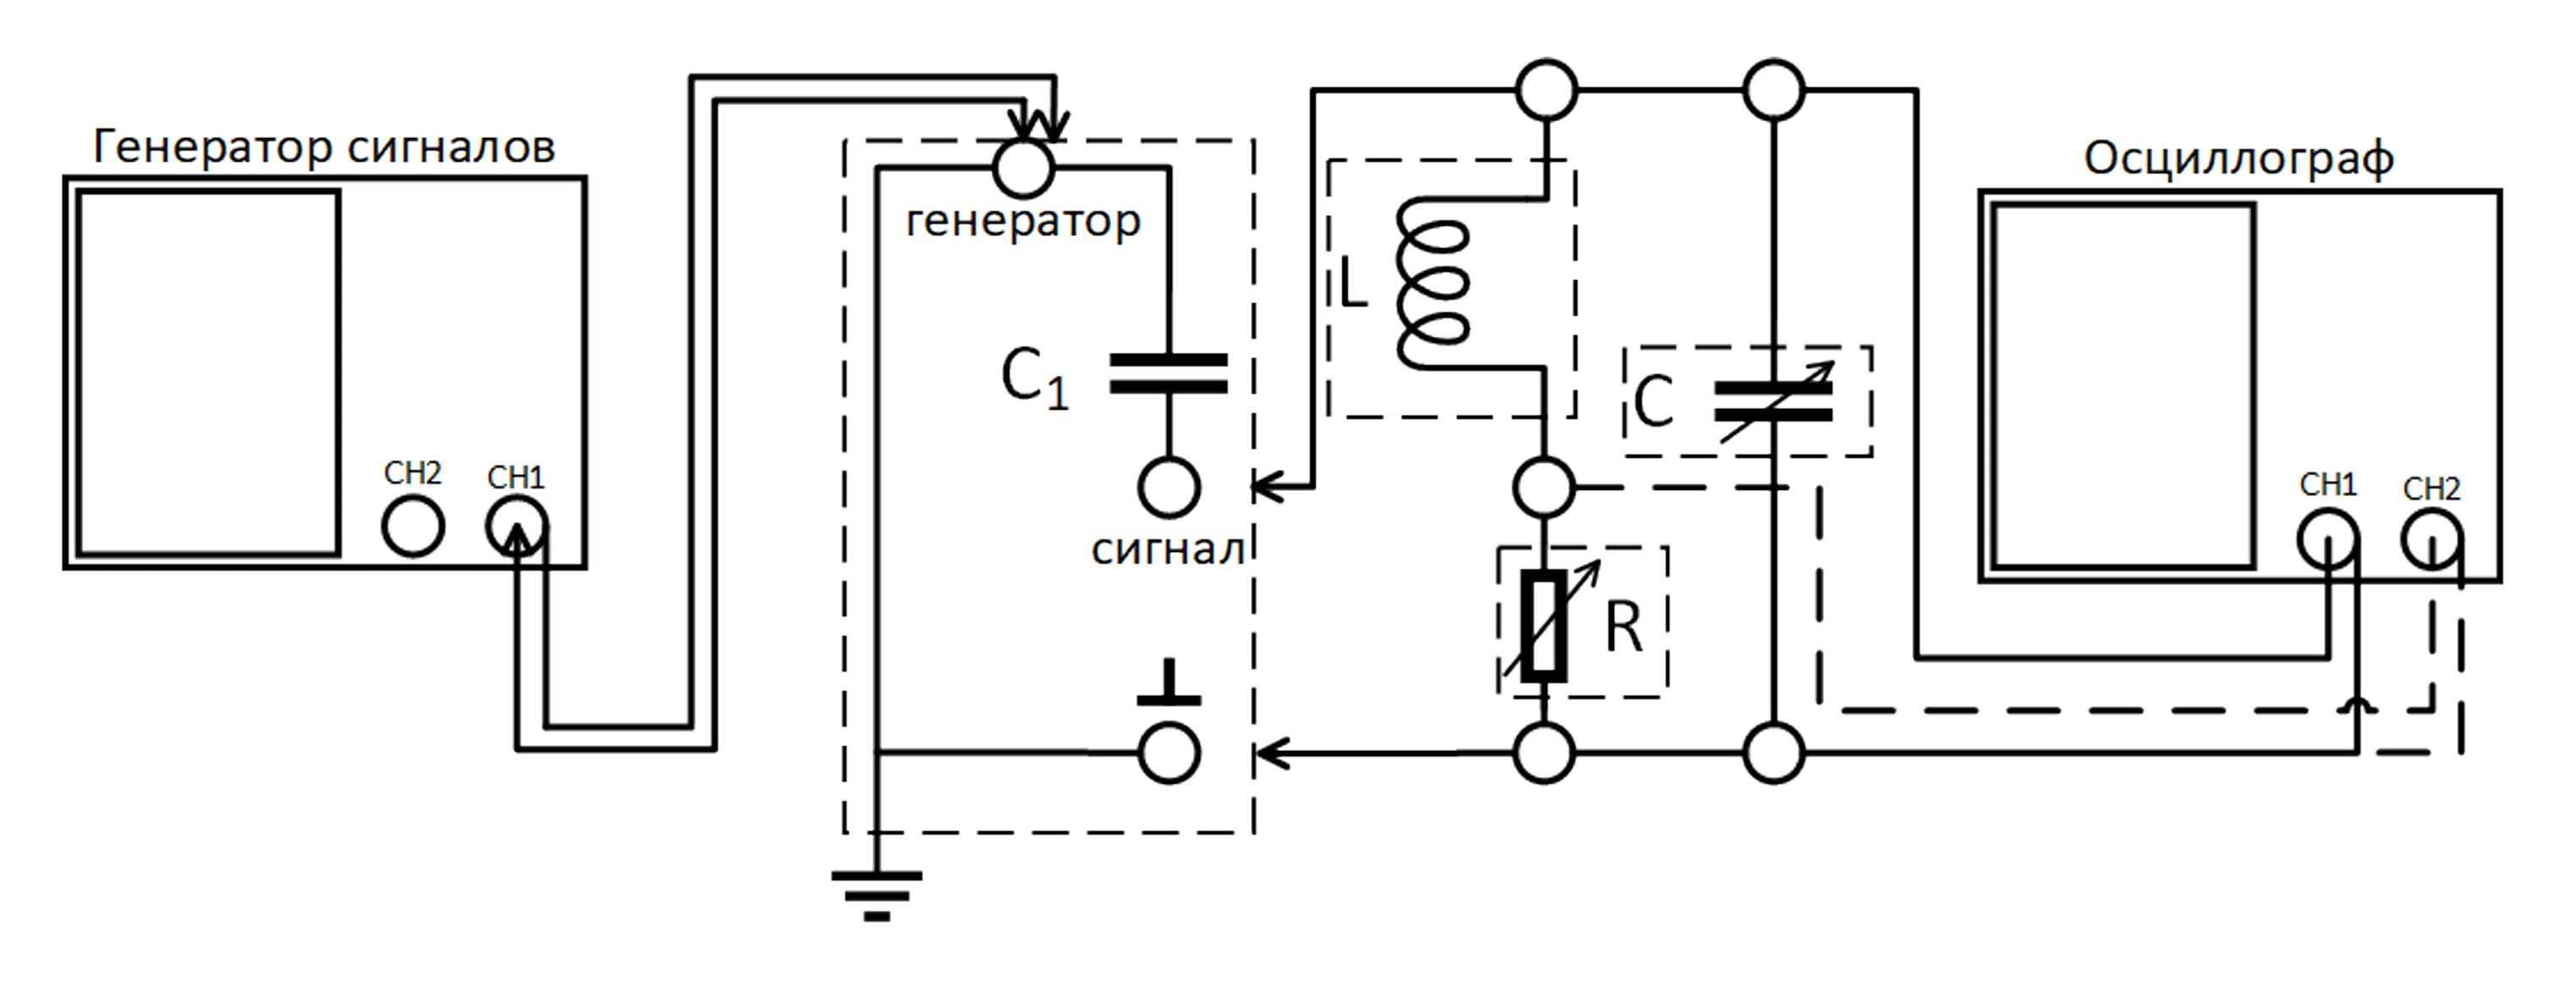
\includegraphics[width=\linewidth]{setup}
    \caption{Схема экспериментальной установки для исследования колебаний.}
    \label{fig:setup}
\end{figure*}

Схема установки показана на рис.~\ref{fig:setup}. Контур собран из катушки индуктивности $L$ (у неё есть собственное сопротивление $R_L$), магазина ёмкостей $C$ и магазина сопротивлений $R$. 

Колебания возбуждаются генератором АКИП-3409/4 через конденсатор связи $C_1$. Его ёмкость выбрана так, чтобы генератор слабо влиял на процессы в контуре. Сигналы наблюдались и записывались двухканальным цифровым осциллографом АКТАКОМ ADS-6124H.

Для свободных колебаний генератор выдаёт короткие прямоугольные импульсы ($10$~мкс), которые заряжают конденсатор $C$, а между импульсами конденсатор разряжается через катушку и резистор. Напряжение $U_C$ подаётся на первый канал осциллографа. Чтобы получить фазовую траекторию, на второй канал подаётся напряжение с резистора $R$ — оно пропорционально току, то есть $dU_C/dt$. 

Для вынужденных колебаний генератор переключается на синусоиду, и, чтобы мерить сдвиг фаз, сигнал генератора одновременно подаётся на второй канал. Установление и затухание колебаний смотрели в режиме цугов (по 15 периодов синусоиды в цуге).



\section{Ход работы}

\subsection{Подготовка приборов к работе и измерение периодов свободных колебаний}

Сначала были настроены приборы. Генератор был подключён напрямую к осциллографу, на нём выставлены прямоугольные импульсы длительностью 10~мкс с частотой повторения 100~Гц и амплитудой 20~В, после чего был подобран уровень синхронизации, чтобы картинка на экране стояла. Затем схема была собрана по рис.~\ref{fig:setup}.

Для начала были установлены $R = 0$~Ом, $L = 100$~мГн и $C = 0$ на магазине. Колебания при этом всё равно затухают — за счёт сопротивления катушки $R_L$. Период измерялся курсорами осциллографа как расстояние между двумя соседними максимумами. Точность ограничена дискретизацией и тем, насколько аккуратно удаётся навести курсор на шумный пик; она оценена в $\pm 0.8$~мкс.

Период $T_0$ при $C = 0$ нужен, чтобы найти паразитную ёмкость $C_0$ — ёмкость катушки, проводов и входа осциллографа, которая есть в схеме всегда. По формуле Томсона
\begin{equation}
    C_0 = \frac{T_0^2}{4\pi^2 L}
\end{equation}
при $T_0 = 66.0$~мкс и $L = 100$~мГн получаем $C_0 = 1.10$~нФ ($0.0011$~мкФ). Относительная погрешность равна $2 \Delta T_0 / T_0$, погрешностью $L$ можно пренебречь (LCR-метр показал $L = 99.944$~мГн, то есть всего на 0.06\,\% меньше номинала). В итоге $C_0 = 1.10 \pm 0.03$~нФ; эта ёмкость в дальнейшем прибавлялась к показаниям магазина.

Затем ёмкость магазина менялась от 0 до 0.009~мкФ с шагом 0.001~мкФ, и для каждого значения записывался период. Погрешность магазина здесь гораздо меньше погрешности курсорных измерений, так что в ошибку $T$ вносит вклад только $\Delta T$. Результаты — в таблице~\ref{tab:periods}.

\begin{table}[h!]
    \caption{Зависимость периода свободных колебаний $T$ от емкости магазина $C$ при $L = 100$~мГн.}
    \label{tab:periods}
    \begin{ruledtabular}
        \begin{tabular}{cc}
            $C$, мкФ & $T$, мкс \\
            \colrule
            0.000 & 66.0 $\pm$ 0.8 \\
            0.001 & 91.6 $\pm$ 0.8 \\
            0.002 & 110.0 $\pm$ 0.8 \\
            0.003 & 128.0 $\pm$ 0.8 \\
            0.004 & 142.0 $\pm$ 0.8 \\
            0.005 & 155.0 $\pm$ 0.8 \\
            0.006 & 168.0 $\pm$ 0.8 \\
            0.007 & 179.0 $\pm$ 0.8 \\
            0.008 & 189.0 $\pm$ 0.8 \\
            0.009 & 199.0 $\pm$ 0.8 \\
        \end{tabular}
    \end{ruledtabular}
\end{table}

\begin{figure*}[t!]
    \centering
    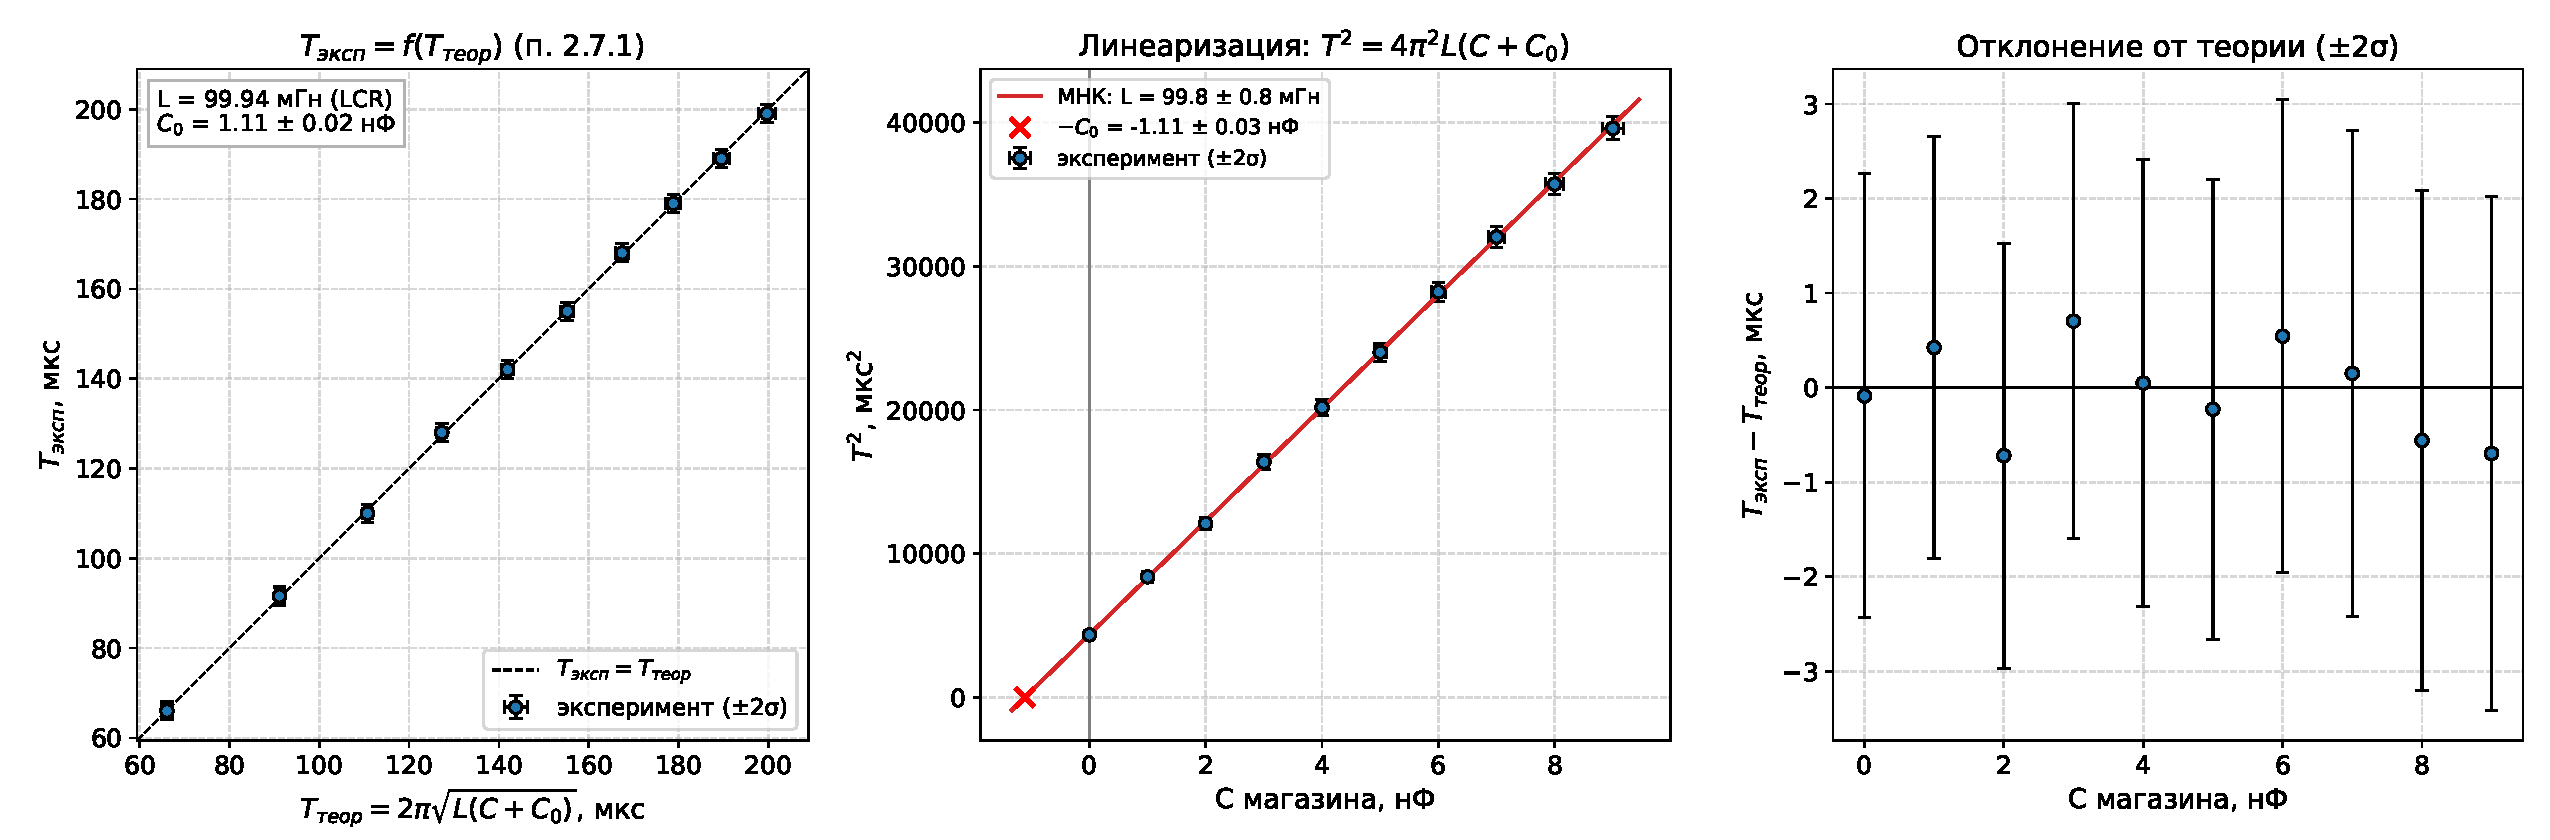
\includegraphics[width=\linewidth]{./period.pdf}
    \caption{Зависимость экспериментального периода от теоретического $T=2\pi\sqrt{L(C+C_0)}$ и линеаризация $T^2(C)$.}
    \label{fig:period}
\end{figure*}

Если построить $T^2$ от $C$ и провести прямую $T^2 = 4\pi^2 L\,(C + C_0)$ (рис.~\ref{fig:period}), получается $L = 99.8 \pm 0.8$~мГн и $C_0 = 1.11 \pm 0.03$~нФ. Это совпадает и с LCR-метром ($99.944$~мГн), и с $C_0$, найденным по одному $T_0$. Экспериментальные периоды отличаются от рассчитанных в среднем на $0.5$~мкс ($0.4\,\%$).


\subsection{Критическое сопротивление и декремент затухания}

При $L = 100$~мГн и резонансной частоте $\nu_0 = 6.5$~кГц нужная ёмкость $C^* = 1 / (4\pi^2 \nu_0^2 L) \approx 6.0$~нФ ($0.006$~мкФ). Для таких параметров критическое сопротивление должно быть $R_{cr, \text{теор}} = 2\sqrt{L/C^*} \approx 8165$~Ом. 

При $C = 0.006$~мкФ сопротивление $R$ постепенно увеличивалось, чтобы поймать момент, когда колебания пропадут. Сделать это на глаз не получилось: амплитуда последних колебаний уменьшается плавно, и чёткого перехода на экране не видно. Поэтому прямое значение $R_{cr}$ не приводится. Наибольшее использованное сопротивление, $R = 2040$~Ом, — это только около $0.25\,R_{cr}$, и колебания там ещё хорошо видны ($\Theta\approx 1.8$). $R_{cr}$ было найдено по декрементам, это описано ниже.

Затем измерялась зависимость декремента $\Theta$ от сопротивления. Для первой оценки амплитуды $U_m$ и $U_{m+n}$, разделённые $n$ периодами, снимались вручную горизонтальными курсорами. Сопротивление менялось от $410$~Ом ($\approx 0.05\,R_{cr}$) до $2040$~Ом ($\approx 0.25\,R_{cr}$).

Погрешность отсчёта амплитуды оценена в $\sigma_U \approx 2$~мВ: это толщина луча и то, насколько точно ставится курсор. Погрешность декремента тогда
\begin{equation}
    \sigma_\Theta = \frac{\sigma_U}{n} \sqrt{ \frac{1}{U_m^2} + \frac{1}{U_{m+n}^2} }
\end{equation}
Поскольку $U_m \gg U_{m+n}$, ошибка почти целиком определяется меньшей амплитудой $U_{m+n}$.

Результаты собраны в таблице~\ref{tab:decrement}. Для опытов с вынужденными колебаниями были выбраны два сопротивления: $R_1 = 410$~Ом и $R_2 = 2040$~Ом.

\begin{table}[h!]
    \caption{Зависимость логарифмического декремента затухания $\Theta$ от сопротивления магазина $R$ при $C = 0.006$~мкФ.}
    \label{tab:decrement}
    \begin{ruledtabular}
        \begin{tabular}{cccccc}
            $R$, Ом & $n$ & $U_m$, мВ & $U_{m+n}$, мВ & $\Theta$ & $\sigma_\Theta$ \\
            \colrule
            410  & 3 & 572 & 176  & 0.393 & 0.004 \\
            600  & 3 & 512 & 100  & 0.544 & 0.007 \\
            800  & 3 & 446 & 56   & 0.692 & 0.012 \\
            1000 & 3 & 398 & 31   & 0.851 & 0.022 \\
            1200 & 2 & 354 & 45   & 1.031 & 0.022 \\
            1500 & 2 & 296 & 23   & 1.277 & 0.044 \\
            1750 & 1 & 258 & 56.4 & 1.520 & 0.036 \\
            2040 & 1 & 213 & 36   & 1.778 & 0.056 \\
        \end{tabular}
    \end{ruledtabular}
\end{table}

\subsection{Свободные колебания на фазовой плоскости и автоматизированная обработка}

\begin{figure*}[t!]
    \centering
    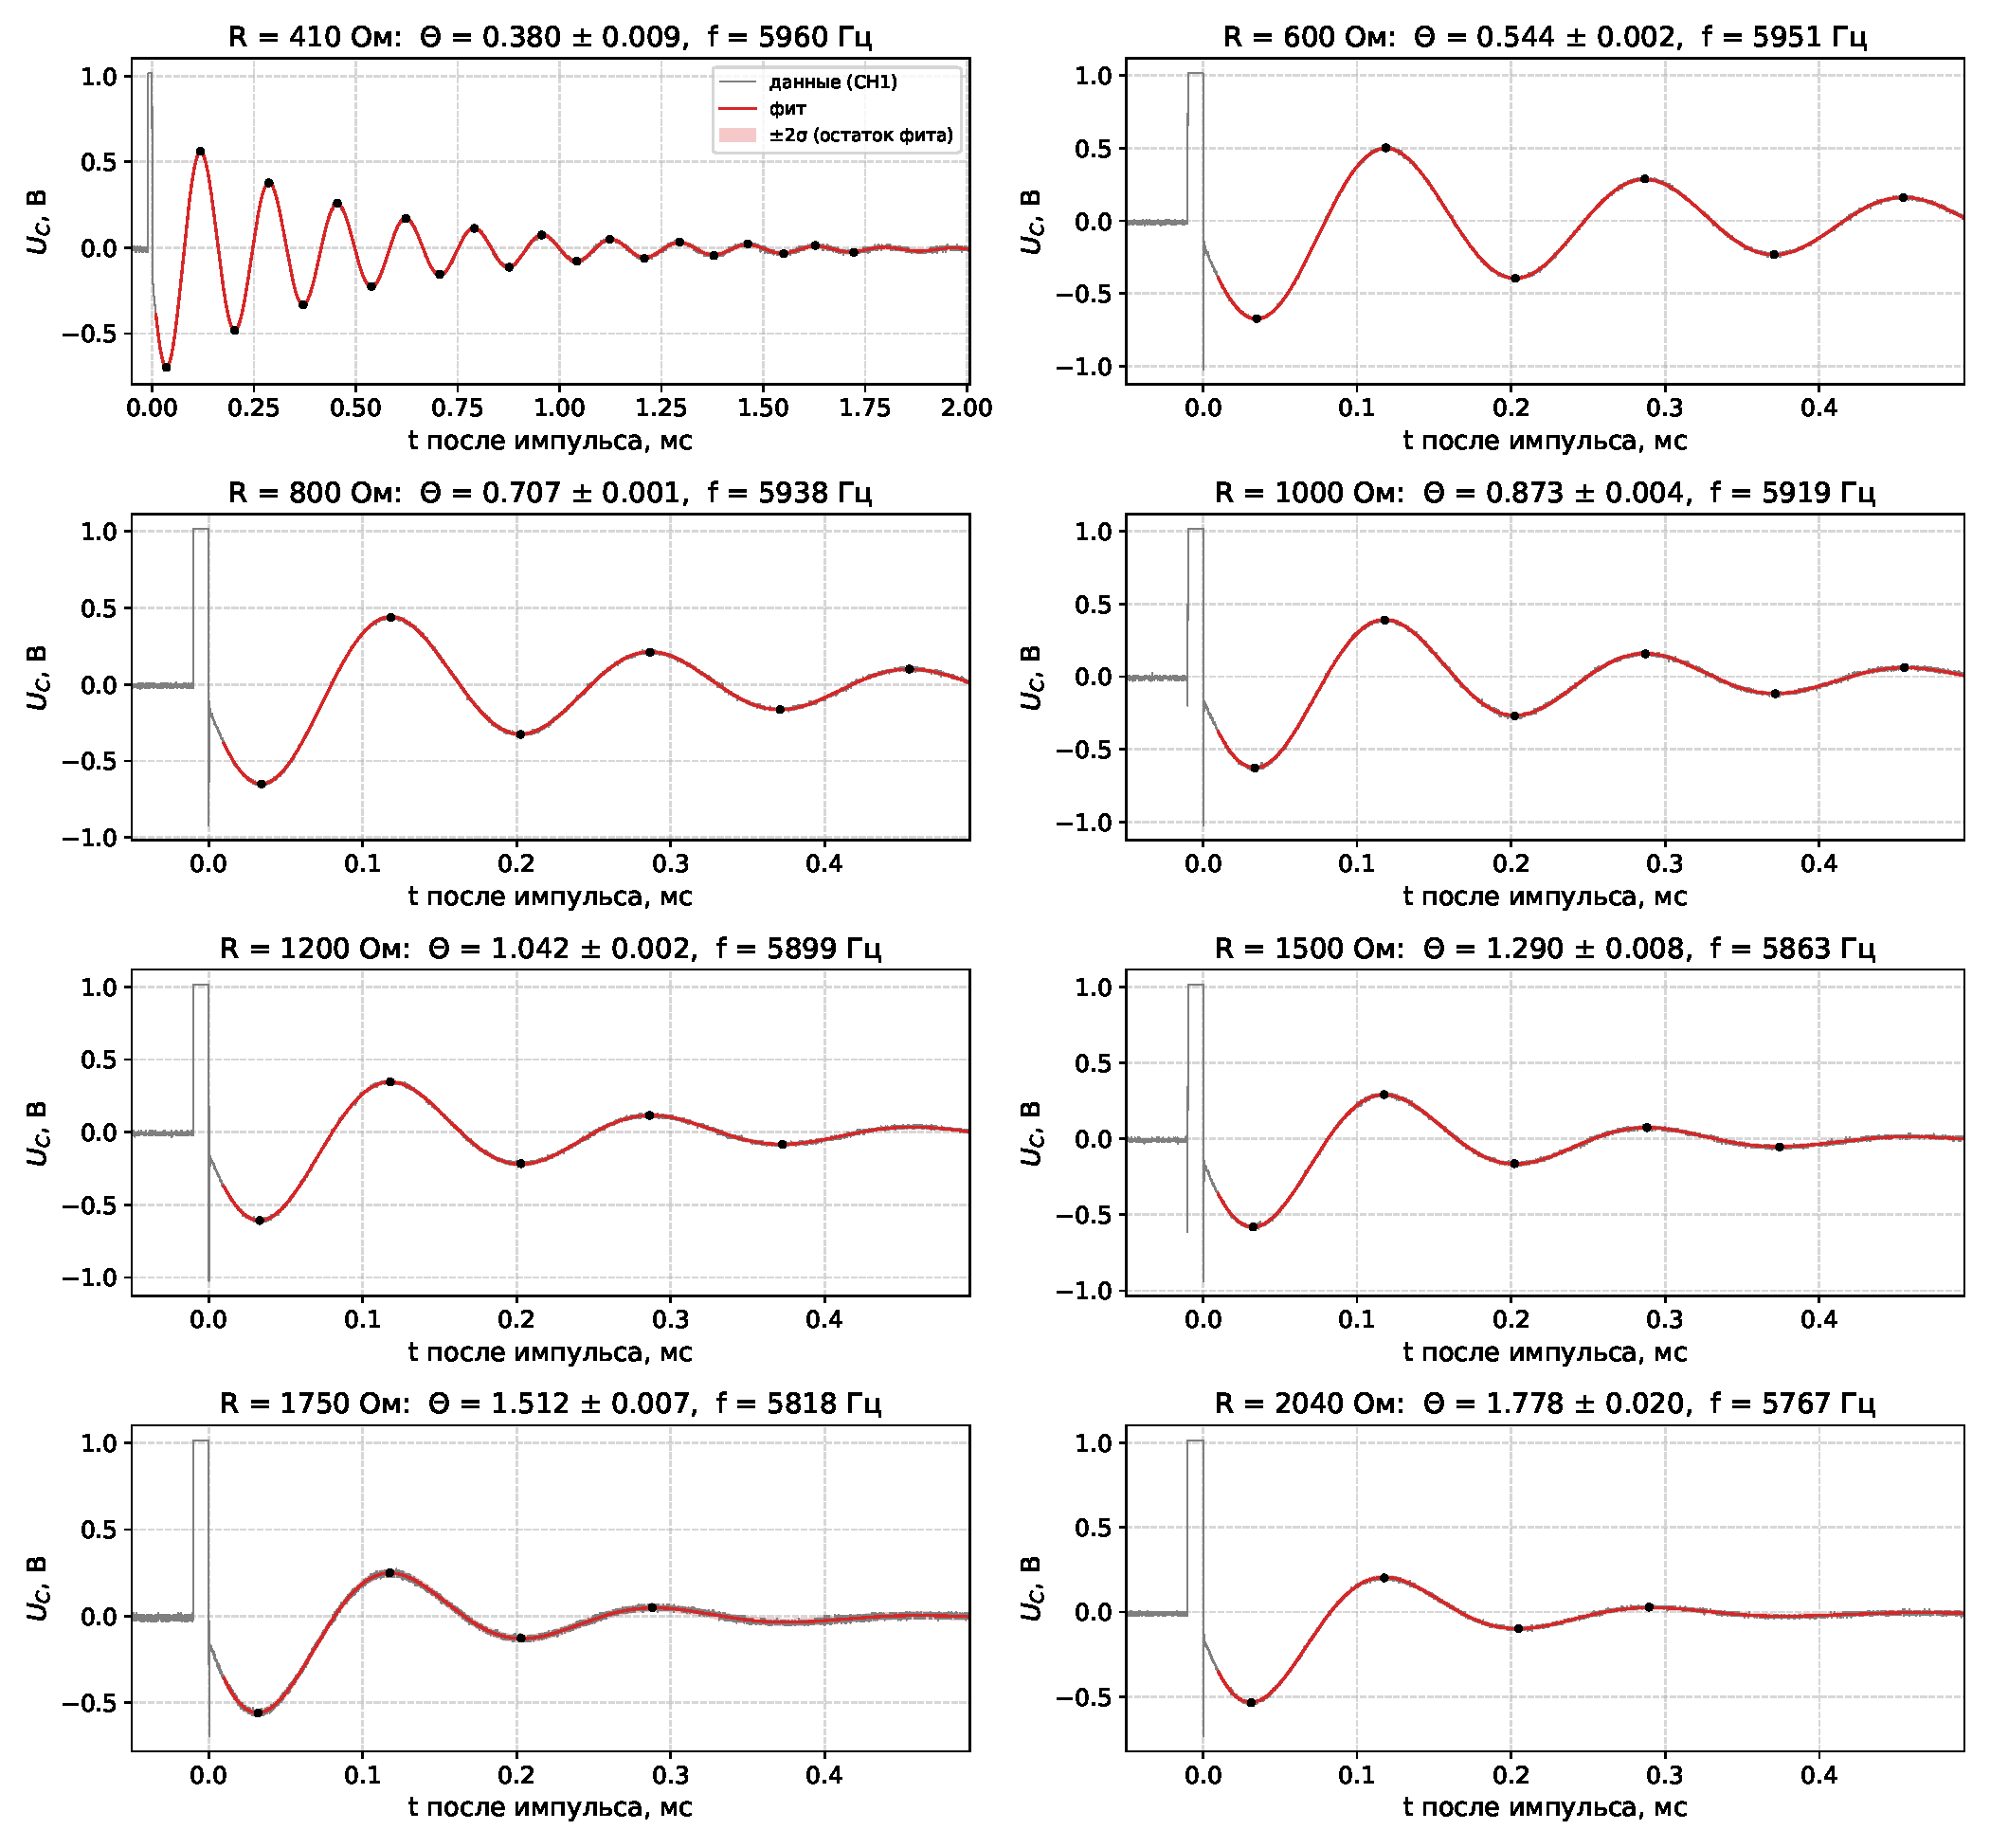
\includegraphics[width=\linewidth]{spiral_waveforms.pdf}
    \caption{Осциллограммы свободных затухающих колебаний напряжения на конденсаторе при различных значениях сопротивления $R$ и их аппроксимация.}
    \label{fig:waveforms}
\end{figure*}

\begin{figure*}[t!]
    \centering
    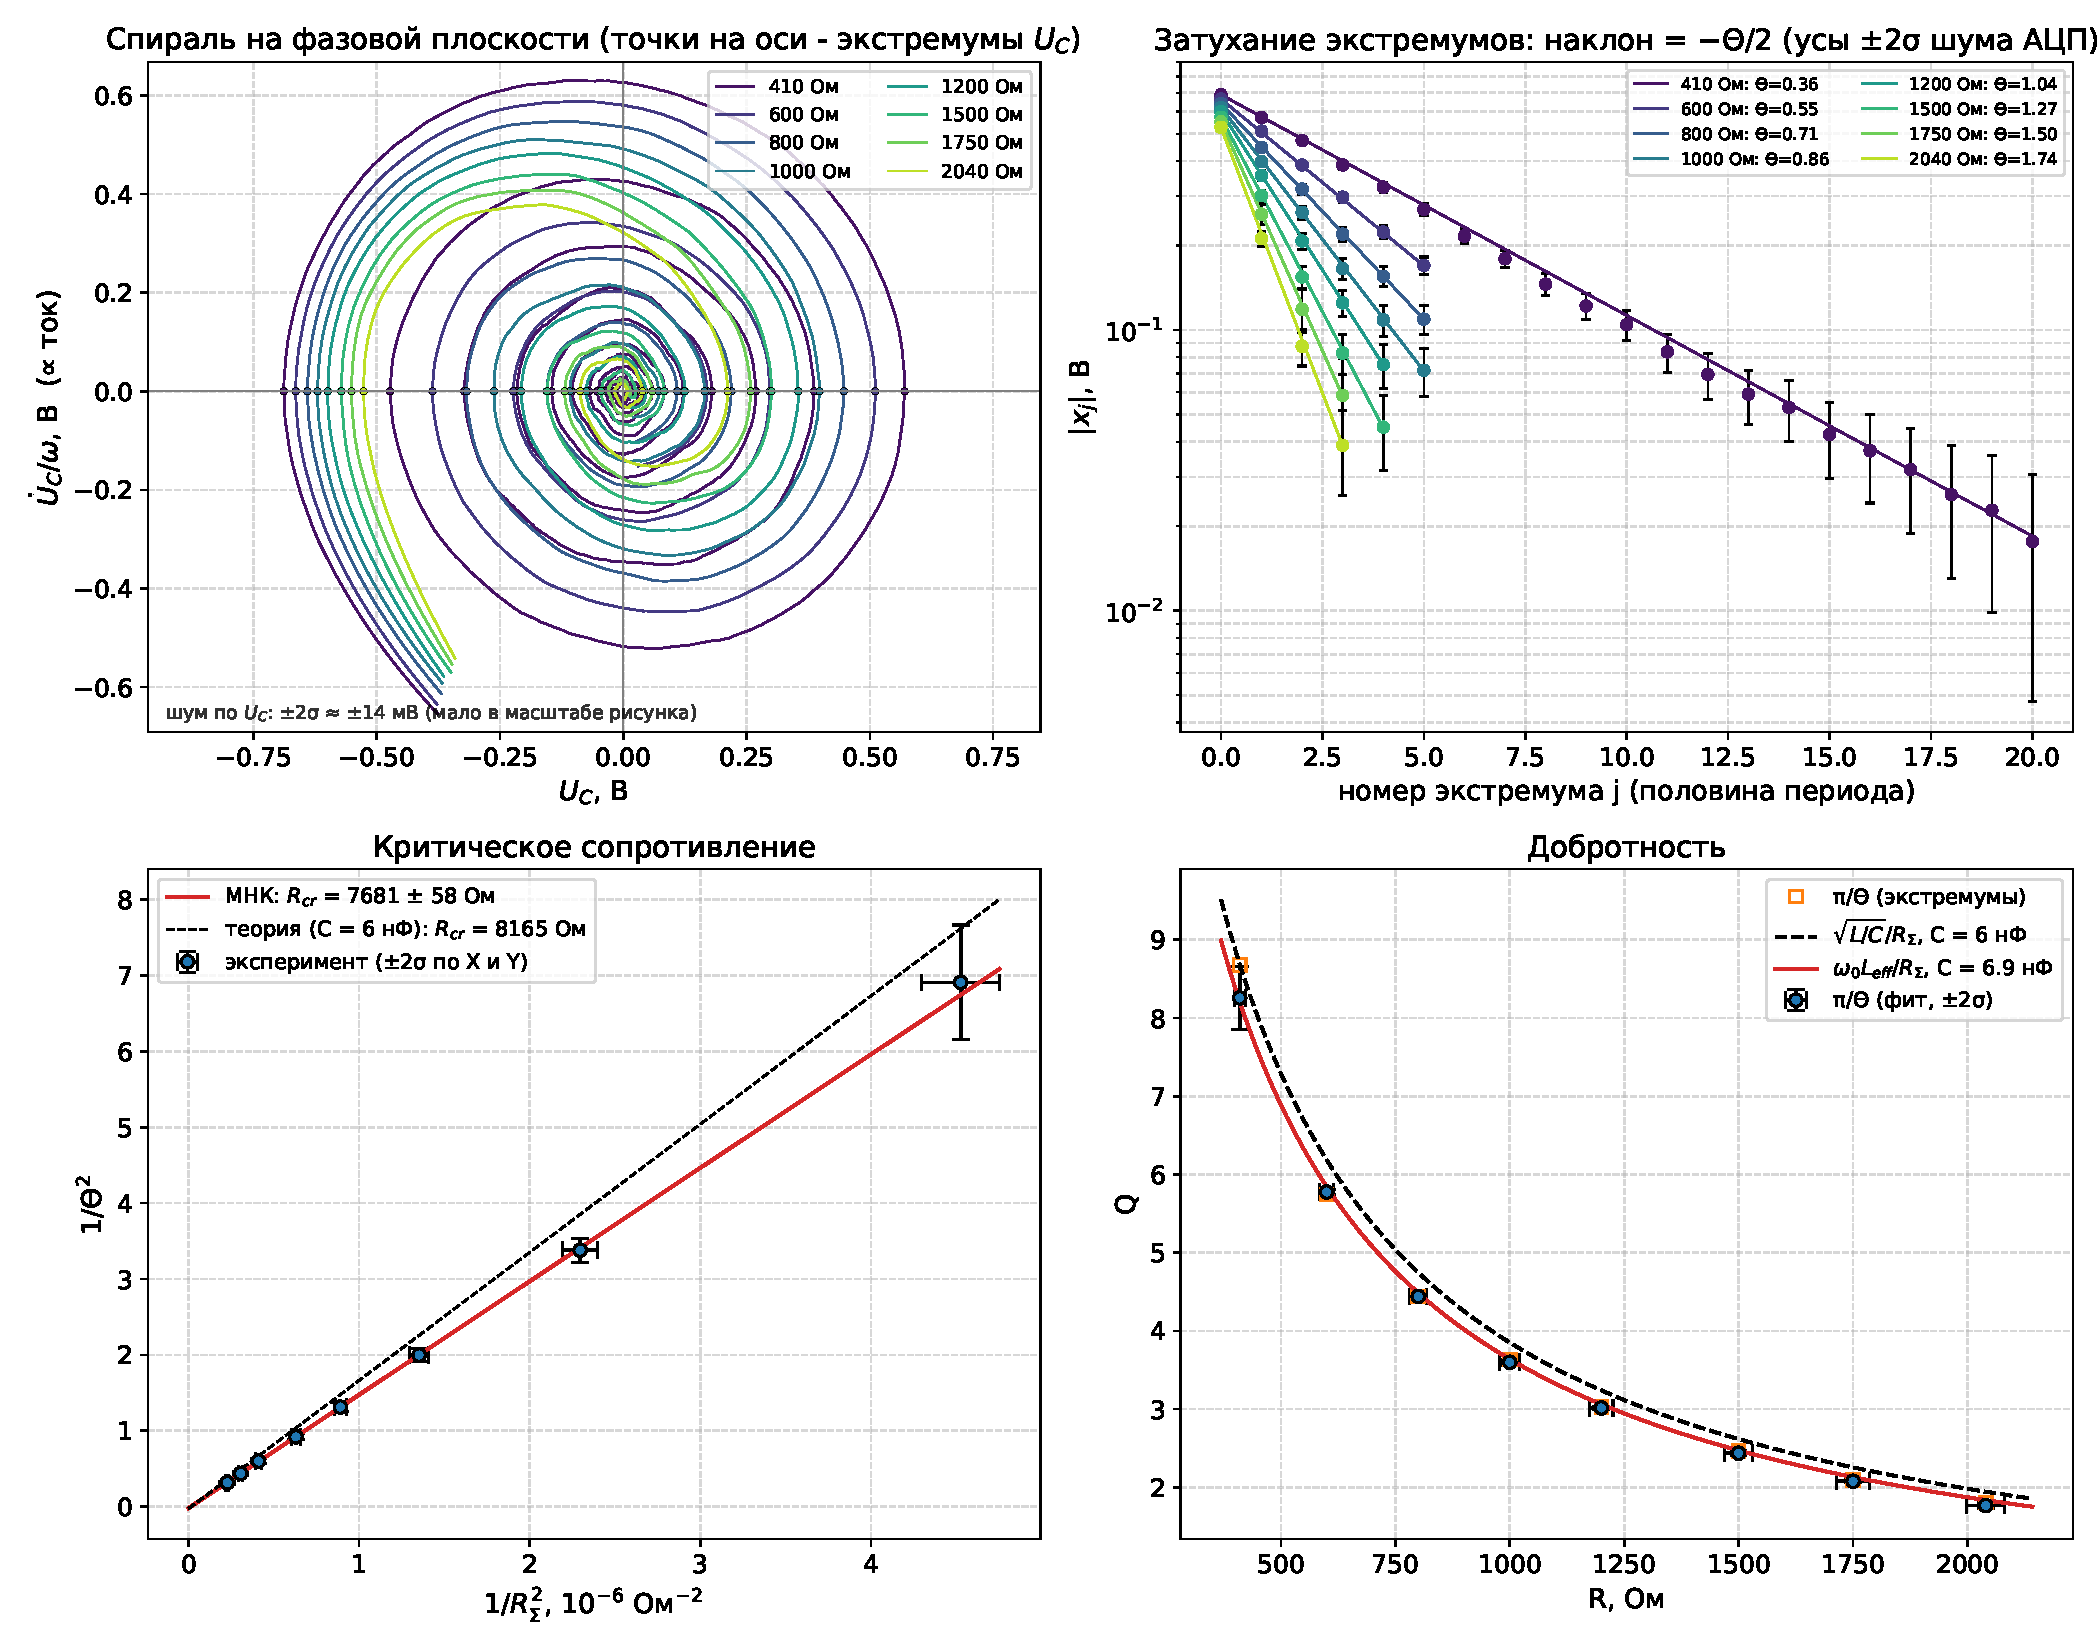
\includegraphics[width=\linewidth]{./spiral_summary.pdf}
    \caption{Результаты автоматизированной обработки: фазовые траектории, затухание экстремумов, линеаризация для поиска $R_{cr}$ и зависимость добротности от сопротивления.}
    \label{fig:summary}
\end{figure*}

Чтобы увидеть фазовую траекторию, осциллограф был переключён в режим X-Y: по горизонтали — напряжение на конденсаторе, по вертикали — напряжение на резисторе, то есть ток. На экране получается спираль, закручивающаяся к началу координат. Чем больше сопротивление (от $0.05~R_{cr}$ до $0.25~R_{cr}$), тем меньше у спирали витков — затухание растёт.

Ручные курсорные измерения дают декремент только по двум точкам, поэтому записанные осциллограммы были дополнительно обработаны на Python (рис.~\ref{fig:waveforms},~\ref{fig:summary}). Каждая запись аппроксимировалась затухающей синусоидой, и по всем точкам сразу находились $\Theta$ и частота $f_d$. Из этой же аппроксимации получено сопротивление катушки $R_L = 60.1 \pm 4.3$~Ом. Напрямую его измерить не удалось: LCR-метр в режиме L/Q показывал <<Q OVER>>. Полное сопротивление контура вычислялось как $R_\Sigma = R + R_L$.

Результаты приведены в таблице~\ref{tab:auto_results}. Погрешность $\Theta$ ($1\sigma$) включает статистическую ошибку фита и разброс, который получается при разном выборе временного окна. Добротность вычислялась как $Q = \pi/\Theta$.

\begin{table}[b!]
    \caption{Параметры затухающих колебаний, полученные в результате автоматизированной обработки осциллограмм.}
    \label{tab:auto_results}
    \begin{ruledtabular}
        \begin{tabular}{ccccc}
            $R$, Ом & $R_\Sigma$, Ом & $f_d$, Гц & $\Theta$ & $Q$ \\
            \colrule
            410  & 470.1  & 5960 & 0.380 $\pm$ 0.009 & 8.26 $\pm$ 0.20 \\
            600  & 660.1  & 5951 & 0.544 $\pm$ 0.002 & 5.78 $\pm$ 0.02 \\
            800  & 860.1  & 5938 & 0.707 $\pm$ 0.001 & 4.44 $\pm$ 0.01 \\
            1000 & 1060.1 & 5919 & 0.873 $\pm$ 0.004 & 3.60 $\pm$ 0.02 \\
            1200 & 1260.1 & 5899 & 1.042 $\pm$ 0.002 & 3.01 $\pm$ 0.01 \\
            1500 & 1560.1 & 5864 & 1.290 $\pm$ 0.008 & 2.44 $\pm$ 0.01 \\
            1750 & 1810.1 & 5818 & 1.512 $\pm$ 0.007 & 2.08 $\pm$ 0.01 \\
            2040 & 2100.1 & 5767 & 1.778 $\pm$ 0.020 & 1.77 $\pm$ 0.02 \\
        \end{tabular}
    \end{ruledtabular}
\end{table}

Добротность сравнивалась с $Q_{\text{теор}} = \frac{1}{R_\Sigma}\sqrt{\frac{L_{eff}}{C_{eff}}}$ (рис.~\ref{fig:summary}, справа внизу). Точки хорошо ложатся на кривую, но надо иметь в виду, что $L_{eff}$, $C_{eff}$ и $R_L$ подобраны по этим же данным. Так что это скорее проверка того, что обработка не противоречит сама себе, чем независимое подтверждение.

Для определения критического сопротивления была построена зависимость $1/\Theta^2$ от $1/R_\Sigma^2$ (рис.~\ref{fig:summary}, слева внизу). Точки ложатся на прямую, и из её наклона получается $R_{cr} = 7681 \pm 58$~Ом.

По номиналам ($L = 100$~мГн, $C = 6.0$~нФ) получалось $8165$~Ом. Фит дал $L_{eff} = 102.7$~мГн и $C_{eff} = 6.90$~нФ (то есть $C_0 \approx 0.90$~нФ), и с ними $2\sqrt{L_{eff}/C_{eff}} = 7715$~Ом — в пределах погрешности с экспериментом. Опять же, это не независимая проверка: $L_{eff}$ и $C_{eff}$ взяты из тех же данных. К тому же в фите они коррелируют, поэтому $C_0 \approx 0.90$~нФ получилось меньше, чем $1.10 \pm 0.03$~нФ по периоду, а $L_{eff}$ на 2.7\,\% больше, чем показал LCR-метр ($99.944$~мГн).


\subsection{Исследование резонансных кривых}

\begin{figure*}[t!]
    \centering
    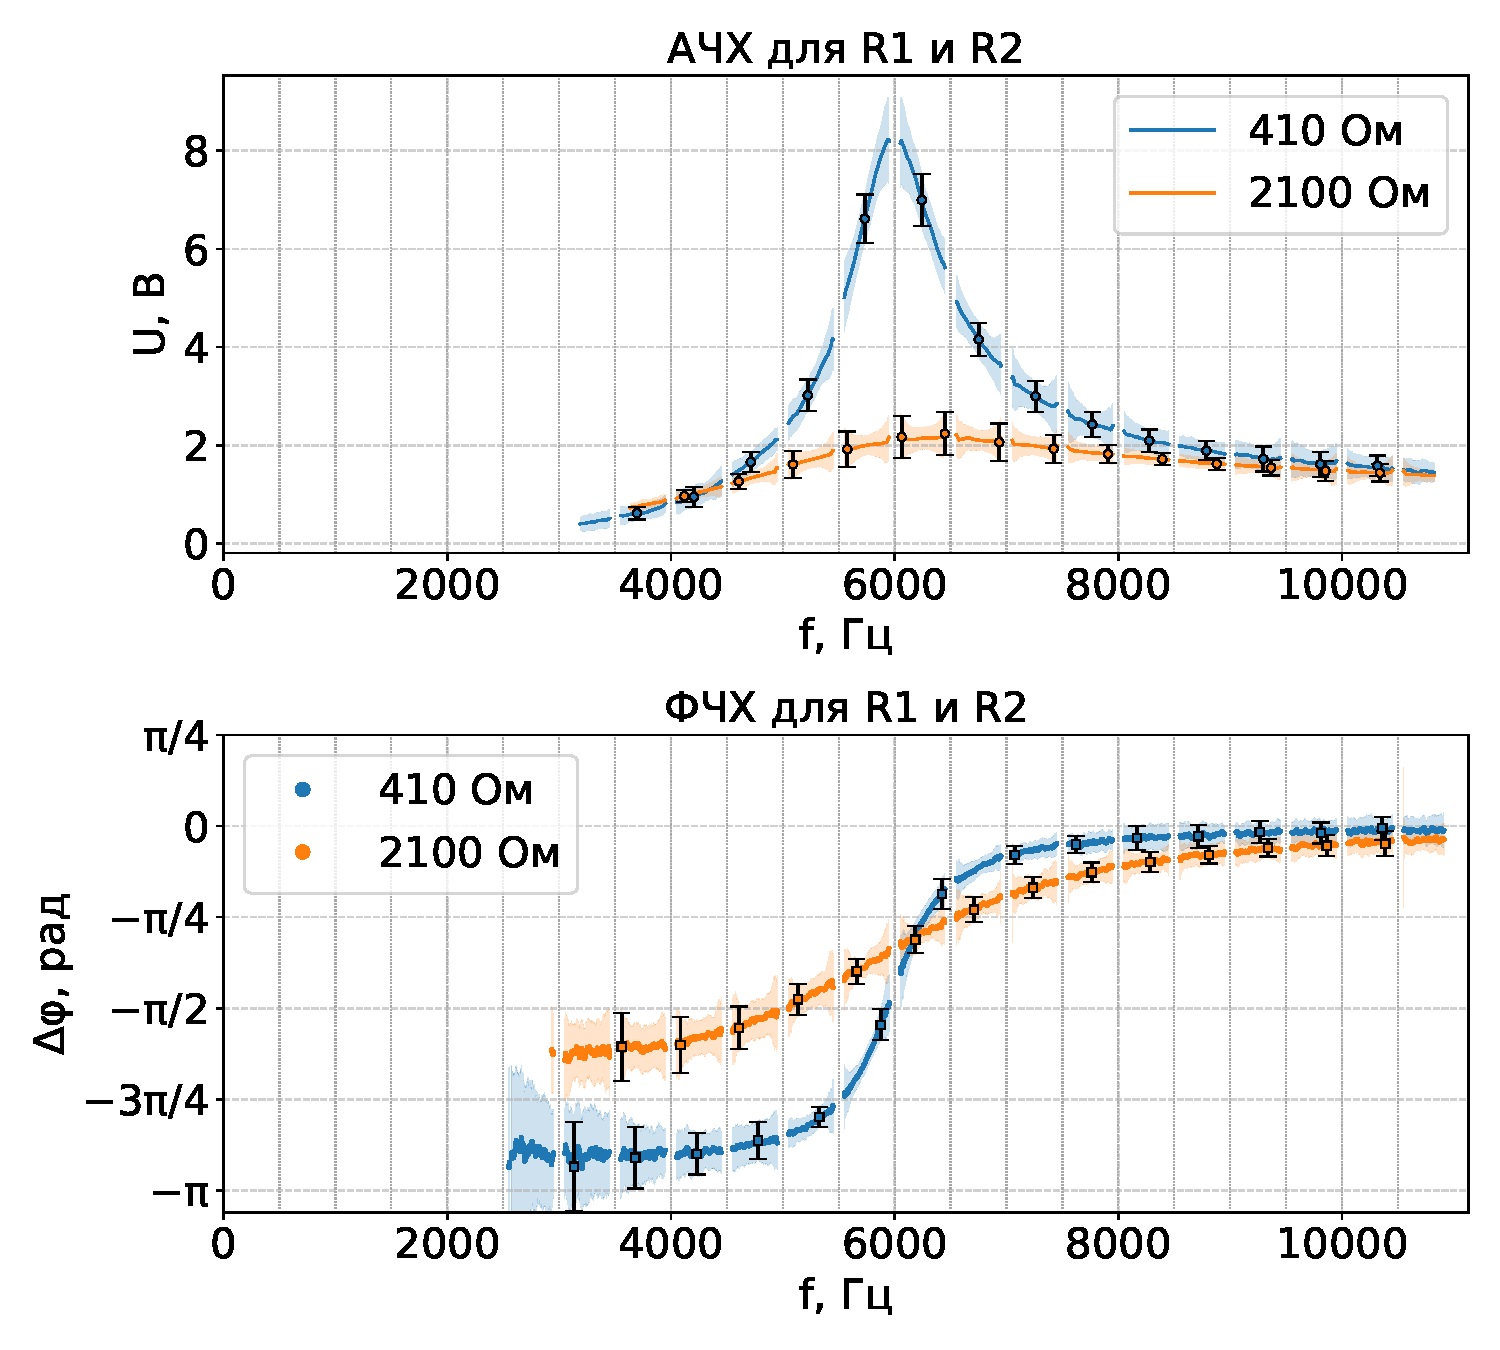
\includegraphics[width=\linewidth]{afc_pfc.pdf}
    \caption{Амплитудно-частотные и фазо-частотные характеристики колебательного контура для двух значений активного сопротивления. Маркерами отмечены выборочные точки с доверительными интервалами $\pm 2\sigma$.}
    \label{fig:afc_pfc}
\end{figure*}

Для вынужденных колебаний осциллограф был возвращён в режим обычной развёртки, в контуре установлены $C = 0.006$~мкФ и сопротивления $R_1$, $R_2$. Вместо ручного измерения амплитуды и сдвига на каждой частоте использовалось качание частоты (sweep): генератор линейно менял частоту от 2990~Гц до 10990~Гц за 10~с, то есть со скоростью 800~Гц/с.

Для АЧХ записывалось напряжение на конденсаторе. Поскольку частота растёт линейно со временем, огибающая записи — это и есть резонансная кривая.

Для ФЧХ сигнал генератора через тройник подавался и на контур, и на один канал осциллографа, а напряжение с конденсатора — на второй. По двум каналам, записанным одновременно, можно найти сдвиг фаз на каждой частоте.

Записи обрабатывались на Python. Огибающая и мгновенная фаза находились через преобразование Гильберта, а разность фаз $\Delta\varphi$ — по произведению аналитического сигнала одного канала на комплексно сопряжённый сигнал другого.

Погрешность амплитуды складывается из разброса огибающей и погрешности вертикального тракта осциллографа (около 3\%). В режиме sweep осциллограф записывал с частотой 1~кГц, поэтому на частотах, кратных 500~Гц, на кривых видны артефакты алиасинга (провалы на АЧХ и вертикальные линии на ФЧХ). Они не вырезались и оставлены на графиках, к физике контура они отношения не имеют. Полученные АЧХ и ФЧХ показаны на рис.~\ref{fig:afc_pfc}.



\subsection{Процессы установления и затухания}

Для наблюдения установления и затухания генератор был переведён в режим цугов (Burst): частота заполнения равна резонансной, в цуге 15 периодов, цуги повторяются каждые 20~мс. На экране видно, как во время цуга амплитуда нарастает до $U_0$, а после его конца колебания свободно затухают. Огибающая затухания выглядит как зеркальное отражение огибающей нарастания.

Измерения проводились при тех же двух сопротивлениях, $R_1 = 410$~Ом и $R_2 = 2040$~Ом. Установившаяся амплитуда составила $U_0^{(1)} = 8.24$~В и $U_0^{(2)} = 2.09$~В.

На участке нарастания снимались пары амплитуд $U_k$ и $U_{k+n}$ через $n$ периодов, и декремент вычислялся по формуле
\begin{equation}
    \Theta_{\text{нар}} = \frac{1}{n} \ln \frac{U_0 - U_k}{U_0 - U_{k+n}}
\end{equation}
Погрешность (с учётом ошибки самого $U_0$):
\begin{equation}
    \begin{split}
    \sigma_{\Theta_{\text{нар}}} = \frac{\sigma_U}{n} \Bigg[ &\frac{1}{(U_0 - U_k)^2} + \frac{1}{(U_0 - U_{k+n})^2} \\
    &+ \left( \frac{1}{U_0 - U_{k+n}} - \frac{1}{U_0 - U_k} \right)^2 \Bigg]^{1/2}
    \end{split}
\end{equation}
где $\sigma_U \approx 0.05$~В — погрешность отсчёта курсором. Хуже всего с амплитудами, близкими к $U_0$: разность $U_0 - U_{k+n}$ становится маленькой, и относительная ошибка резко растёт.

На участке затухания декремент считается как обычно:
\begin{equation}
    \Theta_{\text{зат}} = \frac{1}{n} \ln \frac{U_m}{U_{m+n}}
\end{equation}

Все измерения и посчитанные декременты — в таблицах~\ref{tab:burst_R1} и \ref{tab:burst_R2}. 

\squeezetable
\begin{table}[b!]
    \caption{Процессы нарастания и затухания колебаний при $R_1 = 410$~Ом ($U_0 = 8.24$~В).}
    \label{tab:burst_R1}
    \begin{ruledtabular}
        \begin{tabular}{ccccc|ccccc}
            \multicolumn{5}{c|}{Нарастание} & \multicolumn{5}{c}{Затухание} \\
            $n$ & $U_k$, В & $U_{k+n}$, В & $\Theta_{\text{нар}}$ & $\sigma_{\Theta_{\text{нар}}}$ & $n$ & $U_m$, В & $U_{m+n}$, В & $\Theta_{\text{зат}}$ & $\sigma_{\Theta_{\text{зат}}}$ \\
            \colrule
            1 & 2.84 & 4.48 & 0.36 & 0.02 & 1 & 5.52 & 3.80 & 0.37 & 0.02 \\
            2 & 5.68 & 7.12 & 0.41 & 0.04 & 1 & 2.56 & 1.72 & 0.40 & 0.03 \\
        \end{tabular}
    \end{ruledtabular}
\end{table}

\squeezetable
\begin{table}[b!]
    \caption{Процессы нарастания и затухания колебаний при $R_2 = 2040$~Ом ($U_0 = 2.09$~В).}
    \label{tab:burst_R2}
    \begin{ruledtabular}
        \begin{tabular}{ccccc|ccccc}
            \multicolumn{5}{c|}{Нарастание} & \multicolumn{5}{c}{Затухание} \\
            $n$ & $U_k$, В & $U_{k+n}$, В & $\Theta_{\text{нар}}$ & $\sigma_{\Theta_{\text{нар}}}$ & $n$ & $U_m$, В & $U_{m+n}$, В & $\Theta_{\text{зат}}$ & $\sigma_{\Theta_{\text{зат}}}$ \\
            \colrule
            1 & 0.73 & 1.80 & 1.54 & 0.22 & 1 & 1.82 & 0.32 & 1.74 & 0.16 \\
            2 & 0.73 & 2.04 & 1.65 & 0.70 & 2 & 1.82 & 0.052 & 1.78 & 0.48 \\
        \end{tabular}
    \end{ruledtabular}
\end{table}

Для $R_1 = 410$~Ом средний декремент $\langle\Theta\rangle \approx 0.38$ ($Q\approx 8.3$) — то же, что дали свободные колебания ($\Theta = 0.380 \pm 0.009$). Для $R_2 = 2040$~Ом взвешенные средние $\Theta_{\text{нар}} \approx 1.55 \pm 0.21$ ($Q\approx 2.0$) и $\Theta_{\text{зат}} \approx 1.74 \pm 0.15$ ($Q\approx 1.8$) в пределах погрешности совпадают со спиралью ($\Theta = 1.778 \pm 0.020$). Ошибка $\Theta_{\text{нар}}$ здесь большая: колебания устанавливаются за 1--3 периода, и уже вторая амплитуда почти равна $U_0$.

\subsection{Обработка результатов и анализ добротности контура}

\begin{figure*}[t!]
    \centering
    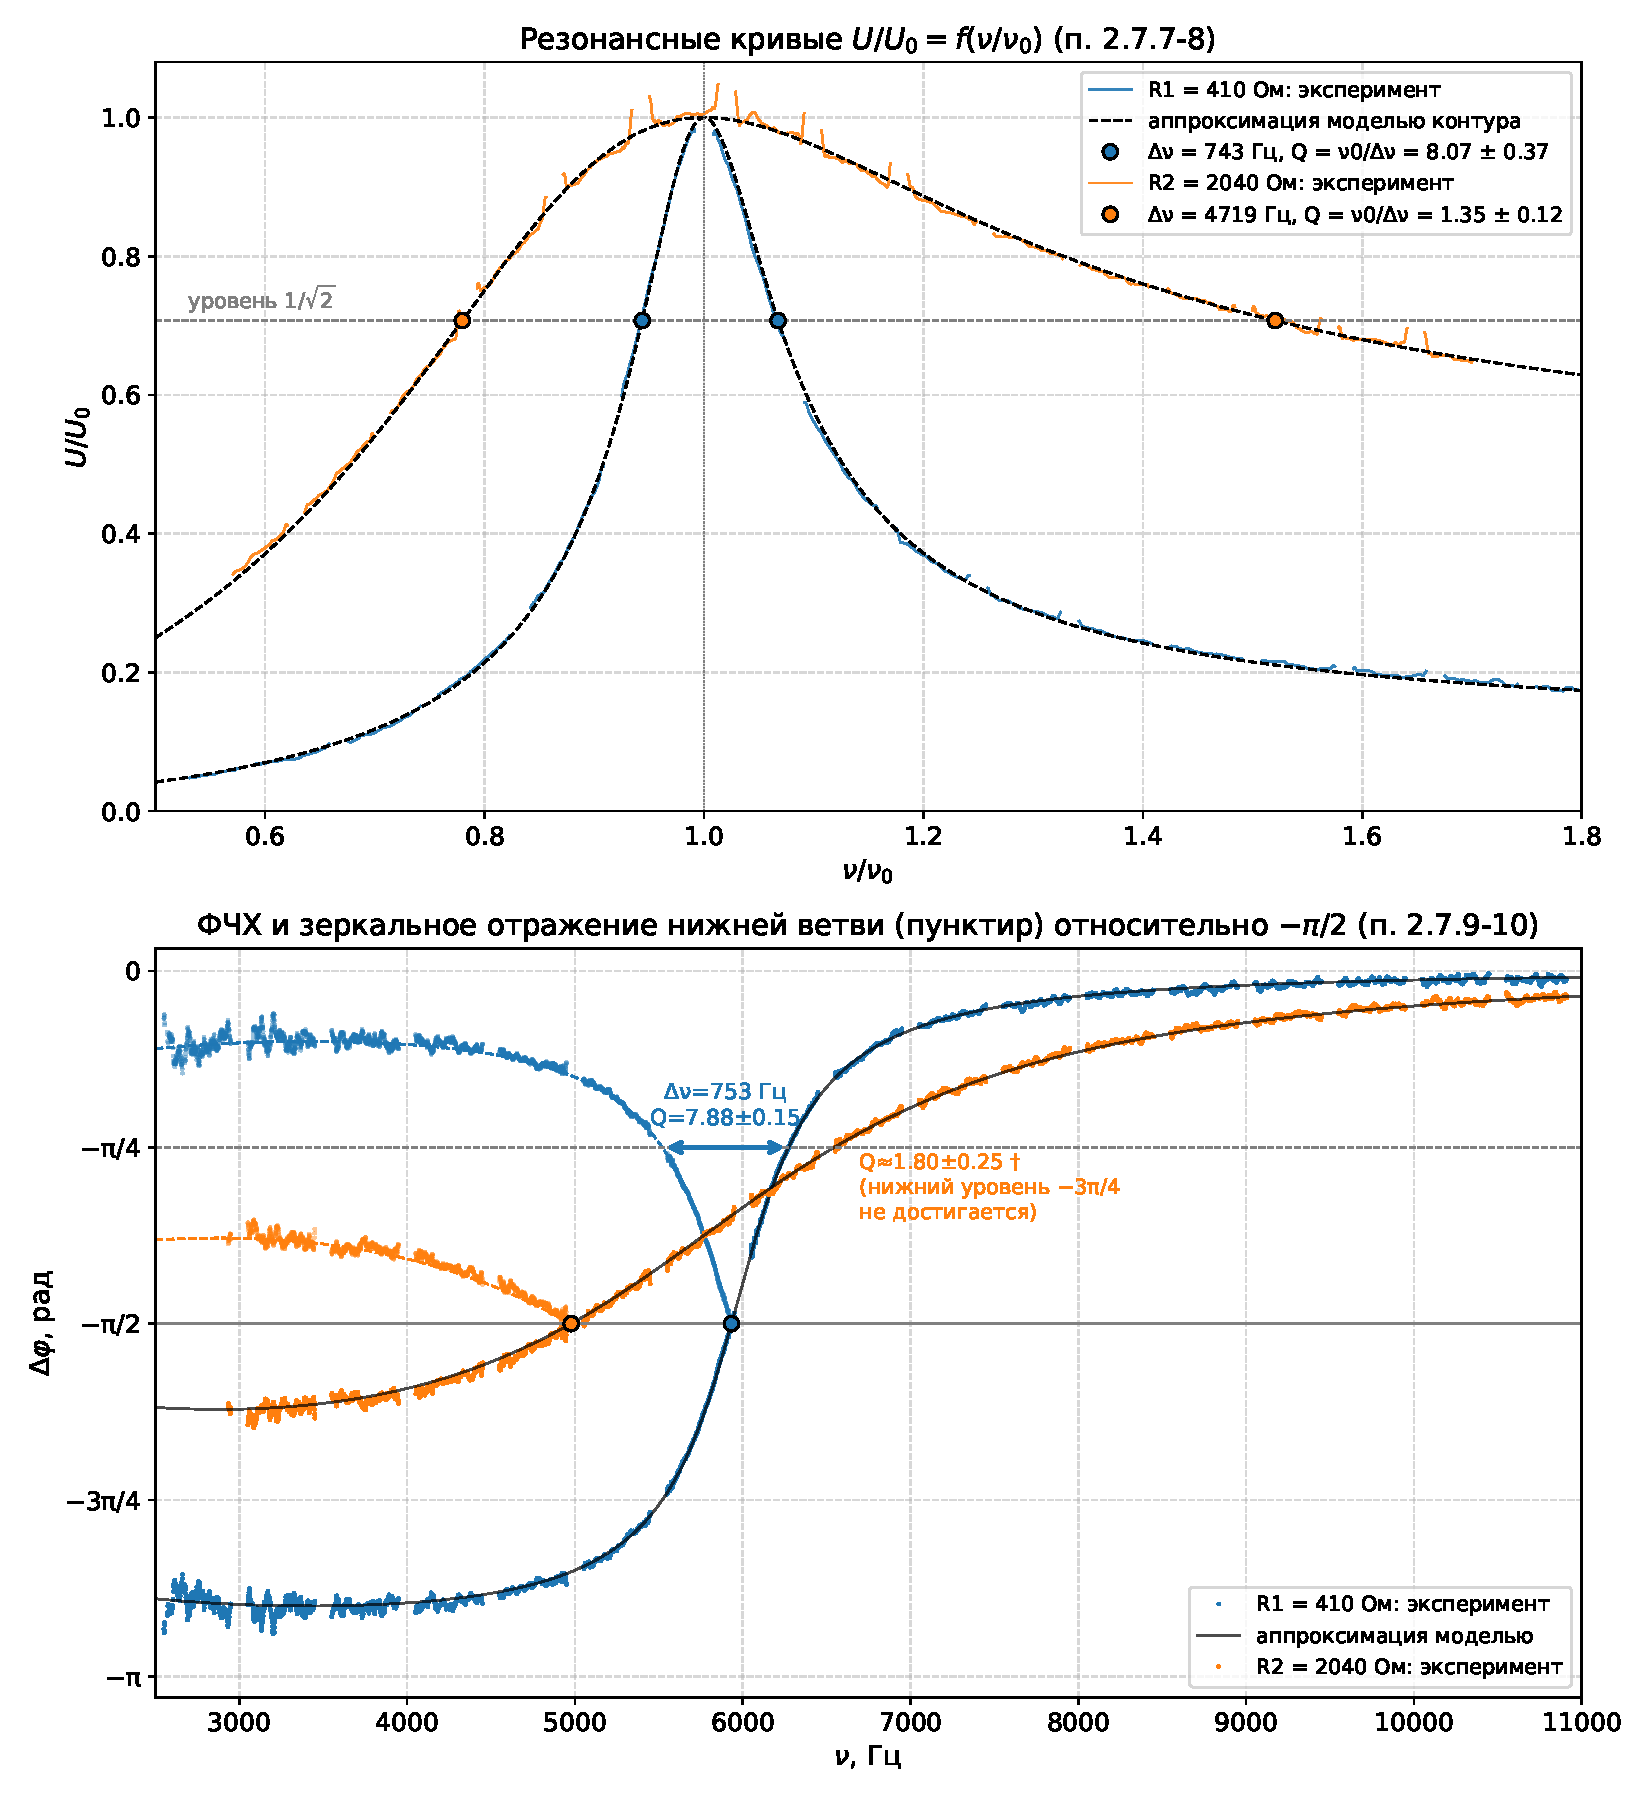
\includegraphics[width=\linewidth]{./q_analysis_curves.pdf}
    \caption{Совместная аппроксимация амплитудно- и фазо-частотных характеристик физической моделью контура. Показаны методы определения ширины резонансных кривых $\Delta\nu$.}
    \label{fig:q_curves}
\end{figure*}


Ниже сведены вместе все способы определения добротности. Теоретически она вычисляется через параметры элементов, $Q_{\text{теор}} = \frac{1}{R_\Sigma}\sqrt{\frac{L}{C}}$. Из свободных колебаний (спираль, фит осциллограмм) и из цугов был получен декремент $\Theta$, а значит и $Q = \pi/\Theta$.

Для вынужденных колебаний АЧХ и ФЧХ аппроксимировались одновременно моделью реального контура (рис.~\ref{fig:q_curves}). Модель учитывает паразитную ёмкость и сопротивление катушки, а на артефакты на частотах, кратных 500~Гц, почти не реагирует. Из фита получено $R_L \approx 51$~Ом. Это на $\approx 2\sigma$ меньше, чем по свободным колебаниям ($60.1 \pm 4.3$~Ом), но $R_L$ в фите коррелирует с другими параметрами, так что такое расхождение допустимо. Погрешности оценивались бутстрапом с учётом шума осциллографа.

По АЧХ $Q = \nu_0 / \Delta\nu$, где $\Delta\nu$ — ширина кривой на уровне $1/\sqrt{2}$ от максимума. По ФЧХ брались частоты, на которых сдвиг фаз равен $-\pi/4$ и $-3\pi/4$ (это то же самое, что ширина на уровне $-\pi/4$ после отражения нижней ветви относительно $-\pi/2$). При $R_2 = 2040$~Ом затухание настолько большое, что фаза до $-3\pi/4$ в исследованном диапазоне частот не доходит. Для этой кривой $Q$ оценивалась по одному уровню $-\pi/4$ с использованием соотношения $\nu_+ \nu_- = \nu_0^2$.

Все значения добротности собраны в табл.~\ref{tab:q_summary}. В пределах погрешностей они согласуются между собой. Выбивается только $Q$ по АЧХ при $R_2$: при $Q \lesssim 2$ резонансная кривая широкая и несимметричная, и формула $\nu_0/\Delta\nu$, выведенная для $Q \gg 1$, даёт заниженное значение.





% выводим все отложенные рисунки/таблицы (иначе revtex теряет табл. с добротностями)
\clearpage
\onecolumngrid
\begin{table}[h!]
    \setlength{\hsize}{\textwidth}\setlength{\columnwidth}{\textwidth}\setlength{\linewidth}{\textwidth}%
    \caption{Добротность контура $Q$, определённая разными способами (погрешности $1\sigma$). Нарастание и затухание: $Q = \pi/\langle\Theta\rangle$ по цугам (взвешенное среднее по двум парам амплитуд, $\sigma_U = 0.05$~В).}
    \label{tab:q_summary}
    \begin{ruledtabular}
        \begin{tabular}{lccccccc}
            $R$, Ом & $\frac{1}{R_\Sigma}\sqrt{L/C}$ & $\pi/\Theta$ (табл.~\ref{tab:auto_results}) & Спираль & АЧХ & ФЧХ & Нарастание & Затухание \\
            \colrule
            $R_1 = 410$  & $8.17 \pm 0.12$ & $8.26 \pm 0.20$ & $8.68 \pm 0.24$ & $8.07 \pm 0.37$ & $7.88 \pm 0.15$ & $8.36 \pm 0.32$ & $8.32 \pm 0.32$ \\
            $R_2 = 2040$ & $1.80 \pm 0.02$ & $1.77 \pm 0.02$ & $1.80 \pm 0.04$ & $1.35 \pm 0.12$ & $1.80 \pm 0.25^{\dagger}$ & $2.02 \pm 0.28$ & $1.80 \pm 0.16$ \\
        \end{tabular}
    \end{ruledtabular}
    \raggedright\footnotesize $^{\dagger}$ Оценка: при $R_2$ фаза не достигает уровня $-3\pi/4$, ширина $\Delta\nu$ найдена по уровню $-\pi/4$ и соотношению $\nu_+\nu_- = \nu_0^2$.
\end{table}
\twocolumngrid

\section{Заключение}
Период свободных колебаний хорошо описывается формулой Томсона $T=2\pi\sqrt{L(C+C_0)}$, отклонения не больше $0.4\,\%$. Паразитная ёмкость установки $C_0 = 1.10 \pm 0.03$~нФ, а индуктивность по графику $T^2(C)$ равна $99.8 \pm 0.8$~мГн, что совпадает с LCR-метром ($99.944$~мГн).

Декремент затухания растёт с сопротивлением: от $0.380 \pm 0.009$ при $R = 410$~Ом до $1.778 \pm 0.020$ при $2040$~Ом. Визуально поймать критическое сопротивление не удалось, но по зависимости $1/\Theta^2$ от $1/R_\Sigma^2$ получено $R_{cr} = 7681 \pm 58$~Ом (по номиналам ожидалось $8165$~Ом). Сопротивление катушки по разным оценкам $51$--$60$~Ом.

Добротность была найдена шестью способами (табл.~\ref{tab:q_summary}). При $R_1 = 410$~Ом все они дают $Q \approx 7.9$--$8.7$, при $R_2 = 2040$~Ом — $Q \approx 1.8$--$2.0$. Исключение — АЧХ при $R_2$ ($1.35 \pm 0.12$): при таком сильном затухании формула $\nu_0/\Delta\nu$ уже не работает. Резонанс наблюдается на $\approx 5.98$~кГц, а не на расчётных $6.5$~кГц, и это тоже объясняется паразитной ёмкостью $C_0$.


% --- Библиография ---
\begin{thebibliography}{99}

\bibitem{practicum2019}
Никулин М. Г., Попов П. В. и др. \textit{Лабораторный практикум по общей физике. Том 2. Электричество и магнетизм.} — М.: МФТИ, 2019.

\bibitem{manual324+5}
\textit{Лабораторная работа 3.2.5 <<Свободные и вынужденные
колебания в электрическом контуре>>.} — МФТИ. \href{https://mipt.ru/upload/%D0%9A%D0%B0%D1%84%D0%B5%D0%B4%D1%80%D0%B0%20%D0%BE%D0%B1%D1%89%D0%B5%D0%B9%20%D1%84%D0%B8%D0%B7%D0%B8%D0%BA%D0%B8/3/lab/%D0%A1%D0%B2%D0%BE%D0%B1%D0%BE%D0%B4%D0%BD%D1%8B%D0%B5%20%D0%B8%20%D0%B2%D1%8B%D0%BD%D1%83%D0%B6%D0%B4%D0%B5%D0%BD%D0%BD%D1%8B%D0%B5%20%D0%BA%D0%BE%D0%BB%D0%B5%D0%B1%D0%B0%D0%BD%D0%B8%D1%8F.pdf}{[Открыть PDF]}

\end{thebibliography}

\end{document}